\DiaryEntry{Groups, Dihedral Groups}{2016-03-15}{Algebra}

These groups \(D_n\) represent the rigid motions of a regular n-sided
polygon. These groups have order \(2n\). We define a clockwise rotation
operation \(r\) as follows:

\begin{figure}[H]
\centering
\includegraphics[scale=0.7]{images/groups_04_1.png}
\caption{Page1}
\end{figure}

And we define a reflection operation \(s\) as in the Figure below
(depending on \(n\) being even or odd, the reflection operation leaves
one or two points unchanged).

\begin{figure}[H]
\centering
\includegraphics[scale=0.7]{images/groups_04_2.png}
\caption{Page1}
\end{figure}

With these two operations, a Diheadral group \(D_n\) is defined as all
products of the two elements \(r\) and \(s\) which satisfy the following
conditions:

\begin{align*}
r^n &= 1 \\
s^2 &= 1 \\
srs &= r^{-1}
\end{align*}


The first condition states, that after \(n\) rotations all polygon
points are back at their original position. The second condition states
that two reflections leave all polygon points unchanged. FInally, the
third condition states, that reflection, rotation, and a reflection is
the same as rotation in the inverse direction.

Note that \(r\) and \(s\) are used to define the group elements; but
\(D_n\) consists of more elements than these two; namely all products
fulfilling above conditions.

\subsection{Example $D_4$}

This group has \(2n = 2 \dot 4 = 8\) elements. The identity element
\(e\), 3 rotations \(r, r^2, r^3\), one reflection \(s\) and 3 rotations
preceded by a reflection \(rs, r^2s, r^3s\). The choice of the last
three elements is somewhat arbitrary (we could have used
\(sr, sr^2, sr^3\)), but choosing it this way is consistent with
\href{http://groupprops.subwiki.org/wiki/Dihedral_group:D8}{this
internet ressource} and the book ``Visual Group Theory'').

The elements are shown in the Figure below.

\begin{figure}[H]
\centering
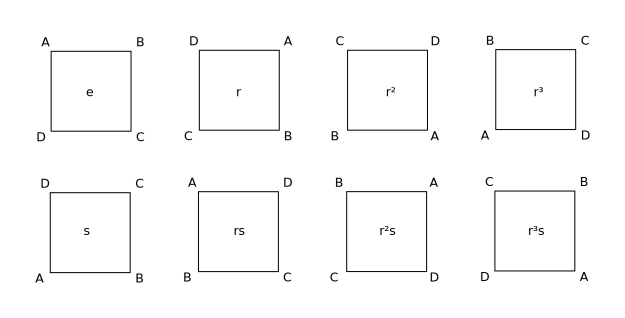
\includegraphics[scale=0.7]{images/groups_04_3.png}
\caption{Page1}
\end{figure}

First note that the group is \textbf{not} abelian.

The multiplication table shall describe the relation between these 8
elements; e.g.~what is the result of \(r^3s \star rs\). This can be
simply written as \(r^3srs\) but this expression is not in the form of
one of the 8 group elements. In order to achieve this, we need to
simplify the resulting expressions so that they equal one of the
elements.

The following multiplication table shows the results of multiplying
elements without simplifying the result. All results in red need further
simplification.

\[
\begin{array}{c|cccccccc}
\star   & 1    & r & r^2  & r^3 & s & rs & r^2s & r^3s \\
\hline
1 & 1 & r & r^2 & r^3 & s & rs & r^2s & r^3s \\
r & r & r^2 & r^3 & 1 & rs & r^2s & r^3s  & s \\
r^2 & r^2 & r^3 & 1 & r & r^2 s & r^3s & s & rs \\
r^3 & r^3 & 1 & r & r^2 & r^3s & s & rs & r^2s \\
s  &  s & \color{red}{sr} & \color{red}{sr^2} & \color{red}{sr^3} & e & \color{red}{srs}  & \color{red}{sr^2s} & \color{red}{sr^3s} \\
rs & rs & \color{red}{rsr} & \color{red}{rsr^2} & \color{red}{rsr^3} & r & \color{red}{rsrs}  & \color{red}{rsr^2s} & \color{red}{rsr^3s} \\
r^2s & r^2s & \color{red}{r^2sr} & \color{red}{r^2sr^2} & \color{red}{r^2sr^3} & r^2 & \color{red}{r^2srs}  & \color{red}{r^2sr^2s} & \color{red}{r^2sr^3s} \\
r^3s & r^3s & \color{red}{r^3sr} & \color{red}{r^3sr^2} & \color{red}{r^3sr^3} & r^3 & \color{red}{r^3srs} & \color{red}{r^3sr^2s} & \color{red}{r^3sr^3s}
\end{array}
\]

In order to simplify the red entries, we observe the following
equalities:

\begin{itemize}
\item
  Start with \(srs = r^{-1}\), left-multiply both sides with \(s\) and
  obtain \(s^2rs = s r^{-1}\) which becomes \(rs = s r^{-1}\).
  Righ-multiplying with \(r\) finally yields \(rsr = s\).
\item
  We have \(sr = r^3 s\): Multiplying on the left with \(r\), we obtain
  \(rsr = r^4 s = r^3\). From the definitions above, we have \(s = s\)
  which is true.
\item
  We have \(sr^2 = r^2s\): Left-multiplying with \(r\) yields
  \(rsr^2 = r^3s\) which we can simplify to \(sr = r^3s\) which was
  proven above.
\item
  We have \(srs = r^{-1}\). Multiplying both sides with \(r^4 = 1\), we
  obtain \(srs = r^3\).
\end{itemize}

The table below shows the simplified expressions based on the identites
above.

\[
\begin{array}{c|cccccccc}
\star   & 1    & r & r^2  & r^3 & s & rs & r^2s & r^3s \\
\hline
1 & 1 & r & r^2 & r^3 & s & rs & r^2s & r^3s \\
r & r & r^2 & r^3 & 1 & rs & r^2s & r^3s  & s \\
r^2 & r^2 & r^3 & 1 & r & r^2 s & r^3s & s & rs \\
r^3 & r^3 & 1 & r & r^2 & r^3s & s & rs & r^2s \\
s  &  s & \color{red}{sr} = r^3s & \color{red}{sr^2} = r^2s & \color{red}{sr^3} = r^2 s r = rs & 1 & \color{red}{srs} = r^3  & \color{red}{sr^2s} = r^2ss = r^2& \color{red}{sr^3s} = ssr = r\\
rs & rs & \color{red}{rsr} = s & \color{red}{rsr^2} = sr = r^3s& \color{red}{rsr^3} = r^2s& r & \color{red}{rsrs} = s^2 = 1  & \color{red}{rsr^2s} = r r^2s s = r^3& \color{red}{rsr^3s} = rs sr = r^2\\
r^2s & r^2s & \color{red}{r^2sr} = rs & \color{red}{r^2sr^2} = r s r = s& \color{red}{r^2sr^3} = r^2 rs = r^3s& r^2 & \color{red}{r^2srs} = r  & \color{red}{r^2sr^2s} = r^2 r^2s s = 1& \color{red}{r^2sr^3s} = r^2ssr = r^3\\
r^3s & r^3s & \color{red}{r^3sr} = r^2s & \color{red}{r^3sr^2} = r^2 rsr r = r^2 s r = rs & \color{red}{r^3sr^3}= r^3 rs = s & r^3 & \color{red}{r^3srs} = r^2& \color{red}{r^3sr^2s} = r^3 r^2ss = r& \color{red}{r^3sr^3s} = r^3ssr = 1
\end{array}
\]

Finally, the table below shows the multiplication table for the dihedral
group \(D_4\):

\[
\begin{array}{c|cccccccc}
\star   & 1    & r & r^2  & r^3 & s & rs & r^2s & r^3s \\
\hline
1 & 1 & r & r^2 & r^3 & s & rs & r^2s & r^3s \\
r & r & r^2 & r^3 & 1 & rs & r^2s & r^3s  & s \\
r^2 & r^2 & r^3 & 1 & r & r^2 s & r^3s & s & rs \\
r^3 & r^3 & 1 & r & r^2 & r^3s & s & rs & r^2s \\
s  &  s & r^3s & r^2s & rs & 1 & r^3  & r^2& r\\
rs & rs & s & r^3s& r^2s & r & 1  & r^3 & r^2\\
r^2s & r^2s & rs & s & r^3s & r^2 & r & 1 & r^3\\
r^3s & r^3s & r^2s & rs & s & r^3 & r^2 & r&  1
\end{array}
\]

The following Figure shows the corresponding Cayley diagram: Red lines
correspond to multiplication with \(r\) and blue lines correspond to
multiplication with \(s\). Since \(s^2 = 1\) the orientation of the blue
lines does \textbf{not} matter: Following a blue line in any direction
\textbf{always} corresponds to multiplication by \(s\) (This is contrary
to multiplication with \(r\) where the direction \textbf{is} important).

Note also that the Cayley diagram uses the (rather unusual) convention
that multiplication is interpreted from left to right; i.e.
\(A \star B\) corresponds to starting in point B, follow the line
corresponding to multiplication with A. This can be seen in the right
part: When we start at \(r\) and follow the blue line to the inner
circle, we land at the point \(sr\) (which is equivalent to \(r^3s\)).

\begin{figure}[H]
\centering
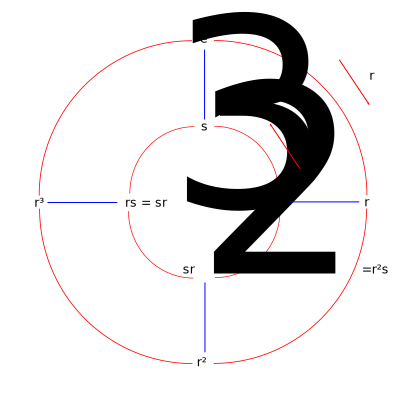
\includegraphics[scale=0.7]{images/groups_04_4.png}
\caption{Page1}
\end{figure}

Using the more common convention that \(AB\) corresponds to starting at
\(A\) and follow the line corresponding to multiplication with \(B\), we
arrive at the Cayle diagram shown below. Again looking at the right part
of the Figure, when we start at \(r\) and follow the blue line to the
inner circle, we land at the point \(rs\).

\begin{figure}[H]
\centering
\includegraphics[scale=0.7]{images/groups_04_5.png}
\caption{Page1}
\end{figure}

\subsubsection{\texorpdfstring{Relation with
\(S_4\)}{Relation with S\_4}}\label{relation-with-s_4}

Contrary to the rigid motions of the triangle (which were equivalent
with \(S_3\)), the group \(D_4\) (and all other groups \(D_n\) with
\(n > 3\)) is a subgroup of \(S_4\). Put another way, \(D_4\) does not
contain all permutations of \(4\) elements like \(S_4\) does. The Figure
below shows 2 missing permutations: the left one is created by twisting
the square along the x-axis; the right one is created by twisting along
the y-axis. Each of these 2 permutations can be rotated and reflected in
8 differerent ways (like discussed above), giving rise to additional
\(2 \times 8 = 16\) elements. Therefore we have \(8 + 16 = 24 = 4!\)
elements; the same number of \(S_4\) has.

\begin{figure}[H]
\centering
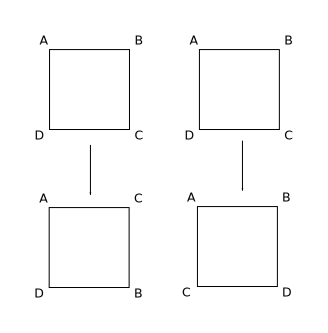
\includegraphics[scale=0.7]{images/groups_04_6.png}
\caption{Page1}
\end{figure}
